\newpage

\section{Projekt platformy}\label{sec:projekt-platformy}

Niniejszy rozdział poświęcony jest platformie sklepu internetowego tulski.com.
Przedmiotem analizy są zarówno komponenty aplikacyjne, jak i infrastrukturalne, które razem tworzą kompletny system e-commerce.

Jak przedstawiono na rysunku~\ref{fig:platform-model}, platforma zawiera moduły do monitoringu, zarządzania certyfikatami, repozytorium obrazów kontenerów, oraz przestrzeń \url{store}, która obejmuje bazę danych, backend, panel administratora oraz witrynę internetową.

Szczegółowy opis i konfiguracja poszczególnych komponentów została przedstawiona w dalszej części rozdziału.

\begin{figure}[p]
    \centering
    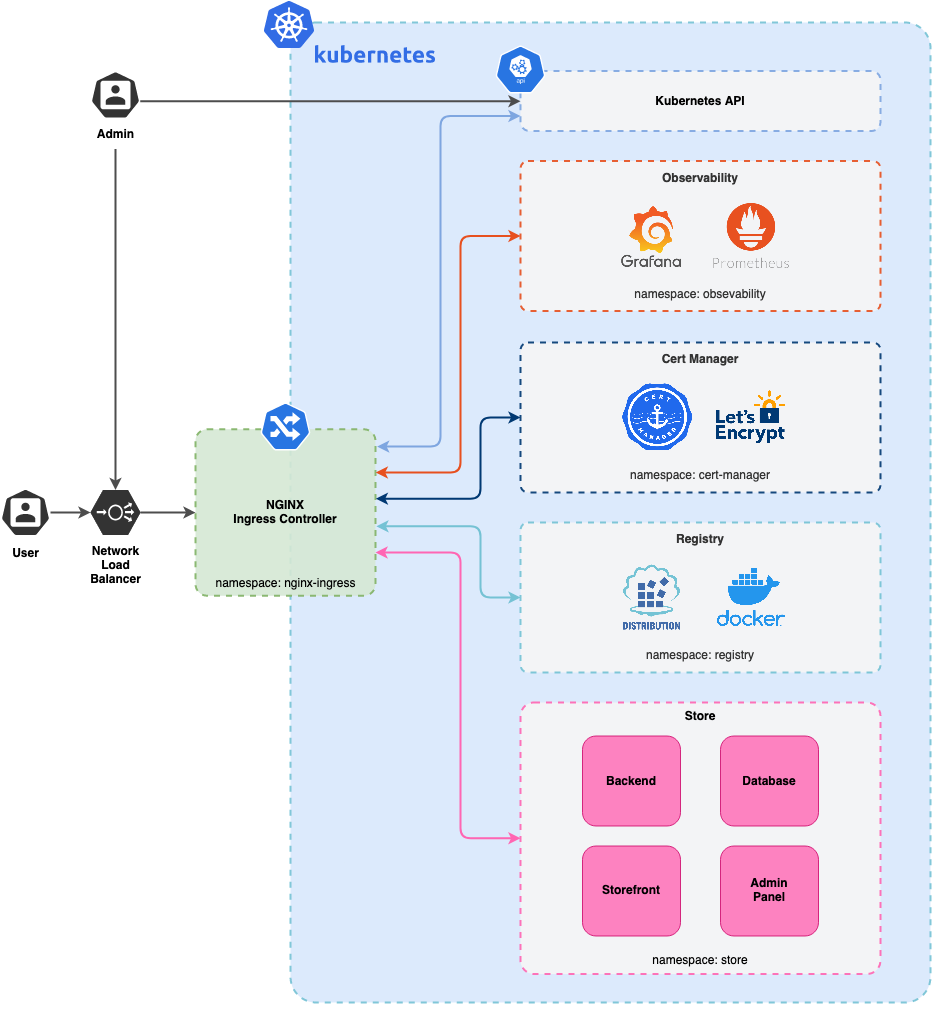
\includegraphics[width=\textwidth]{img/main-infra-model}
    \caption{Model platformy sklepu internetowego tulski}
    \label{fig:platform-model}
\end{figure}

\subsection{Platforma wdrożeniowa}\label{subsec:platforma-wdrozeniowa-kubernetes}

Platformą wdrożeniową dla projektu jest infrastruktura w postaci klastra Kubernetes uruchomionego w chmurze Oracle Cloud Infrastructure.
Klaster składa się z czterech węzłów, każdy wyposażony w 1 procesor Oracle CPU oraz 6 GB pamięci RAM\@.
W skład infrastruktury wchodzi również Network Load Balancer, który dystrybuuje ruch sieciowego pomiędzy węzłami klastra.
Wszystkie elementy infrastruktury zostały zaprojektowanie i wdrożone zgodnie z instrukcjami zawartymi w załączniku~\ref{sec:instrukcja-stworzenia-klastra-kubernetes}.

\subsection{Ingress Controller}\label{subsec:ingress-controller}

Zastosowano NGNIX Ingress Controller, czyli jedną z najpopularniejszych implementacji interfejsu Ingress w środowisku Kubernetes.
Przy użyciu polecenia Helm (zob. listing~\ref{lst:helm-install-ingress-controller}) zainstalowano pakiet \url{oci://ghcr.io/nginxinc/charts/nginx-ingress} w wersji 1.0.2.
NGINX Ingress Controller działa jako DaemonSet, co oznacza uruchomienie jednej instancji na każdym z węzłów klastra.
Dodano integrację z Cert-Manager do zarządzania certyfikatami TLS\@.

\begin{listing}[H]
    \begin{minted}{bash}
helm install ingress-nginx \
    --version 1.0.2 \
    --set controller.kind="daemonset" \
    --set controller.hostNetwork=true \
    --set controller.ingressClass.name="public" \
    --set controller.service.create=false \
    --set controller.enableCertManager=true \
    -n ingress-nginx \
    --create-namespace \
    oci://ghcr.io/nginxinc/charts/nginx-ingress
    \end{minted}
    \caption{Polecenie instalujące pakiet oci://ghcr.io/nginxinc/charts/nginx-ingress}
    \label{lst:helm-install-ingress-controller}
\end{listing}

\newpage

\subsection{Konfiguracja DNS}\label{subsec:konfiguracja-dns}

W konfiguracji DNS platformy tulski zastosowano usługi Cloudflare, dodając pięć rekordów A (admin, api, monitoring, registry, store), wszystkie kierujące na publiczny adres IP Load Balancera.
Wszystkie rekordy korzystają z Cloudflare Proxy.

\begin{figure}[H]
    \centering
    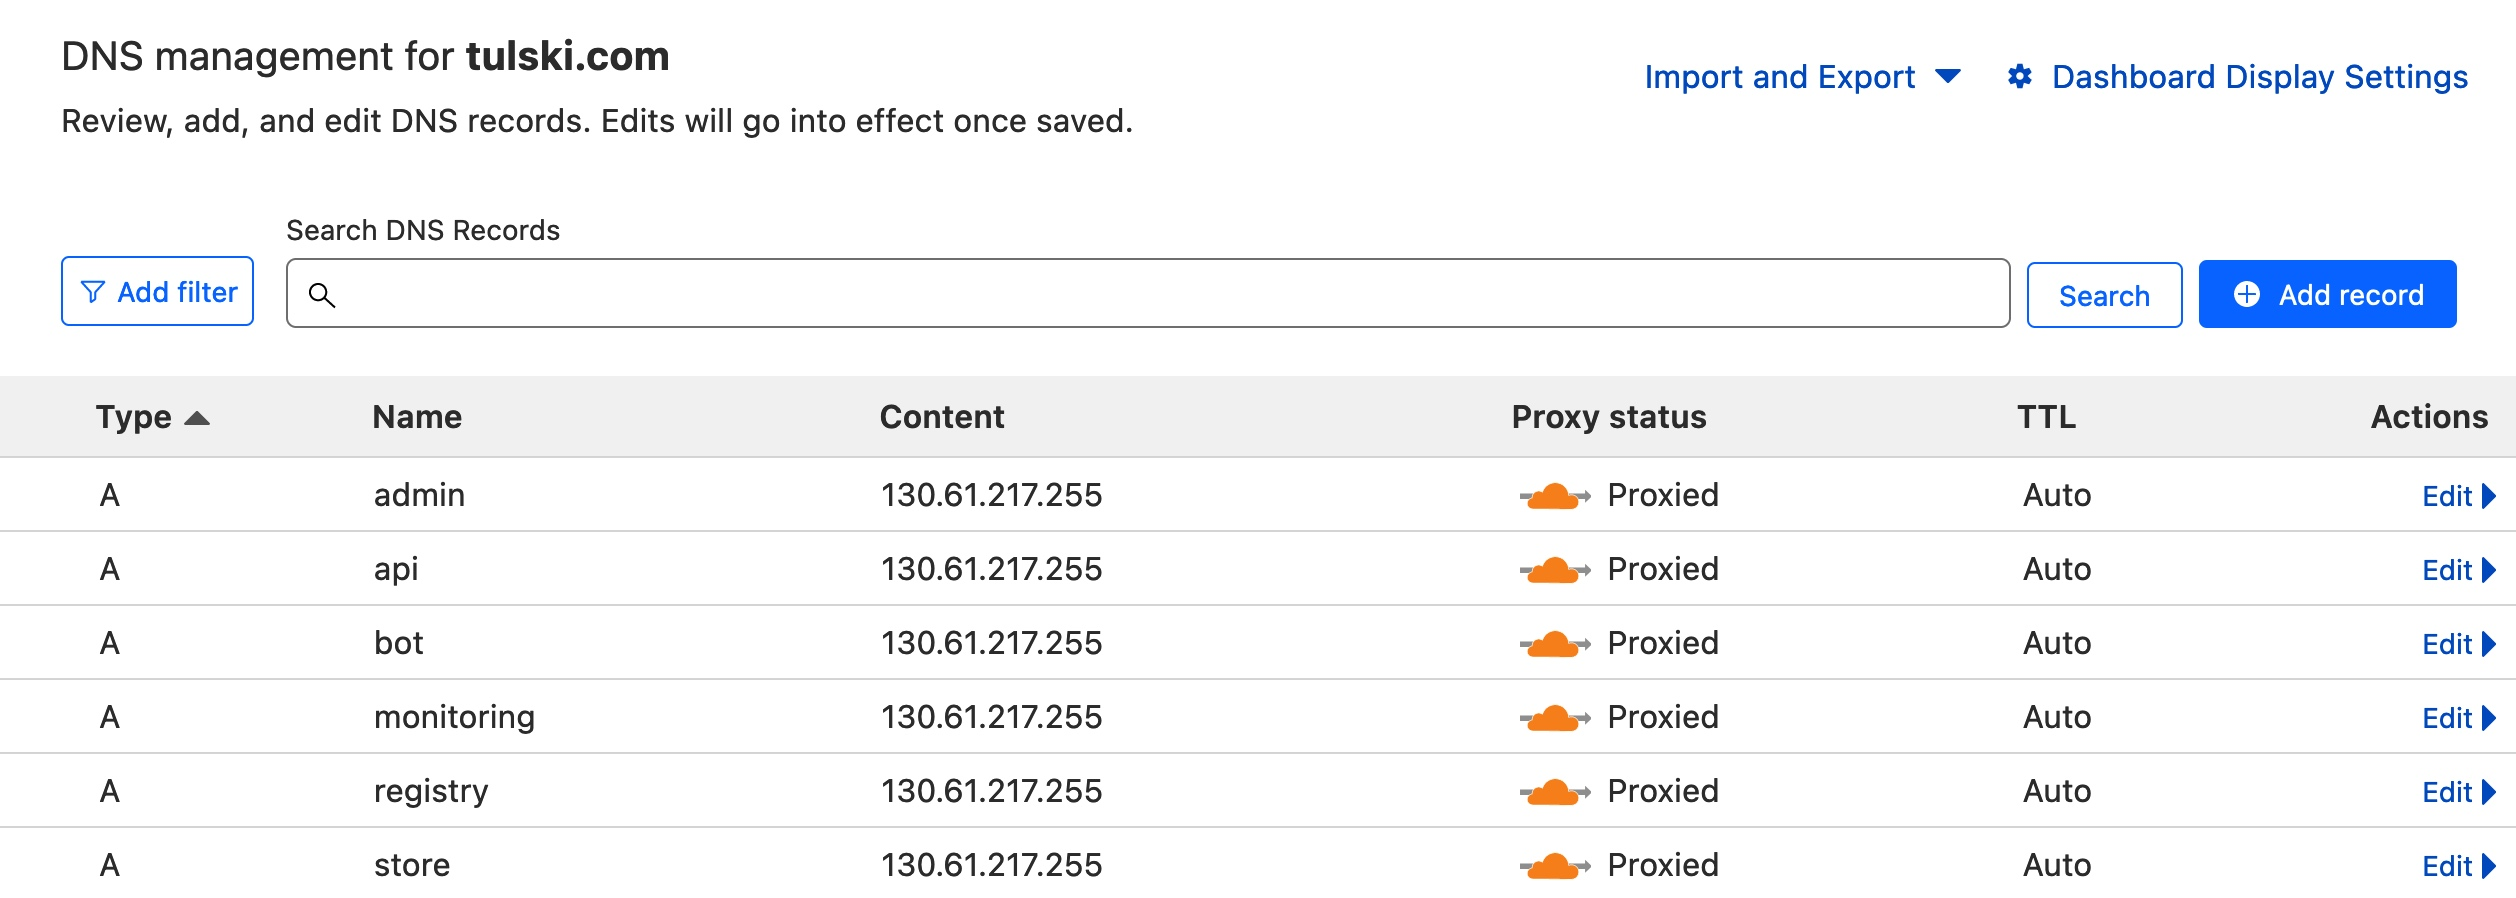
\includegraphics[width=\textwidth]{img/dns-tulski-com}
    \caption{Tabela rekordów DNS dla domeny tulski.com}
    \label{fig:dns-tulski-com}
\end{figure}

\subsection{Monitoring}\label{subsec:monitoring}

\todo{Observability Plane}

\begin{listing}[H]
    \begin{minted}{bash}
helm install observability \
    -f observability/values.yaml \
    --set "grafana.adminPassword=<adminPassword>" \
    -n observability \
    --create-namespace \
    prometheus-community/kube-prometheus-stack
    \end{minted}
    \caption{Polecenie instalujące pakiet prometheus-community/kube-prometheus-stack}
    \label{lst:helm-install-observability}
\end{listing}

%\begin{figure}[p]
%    \begin{figure}[H]
%        \centering
%        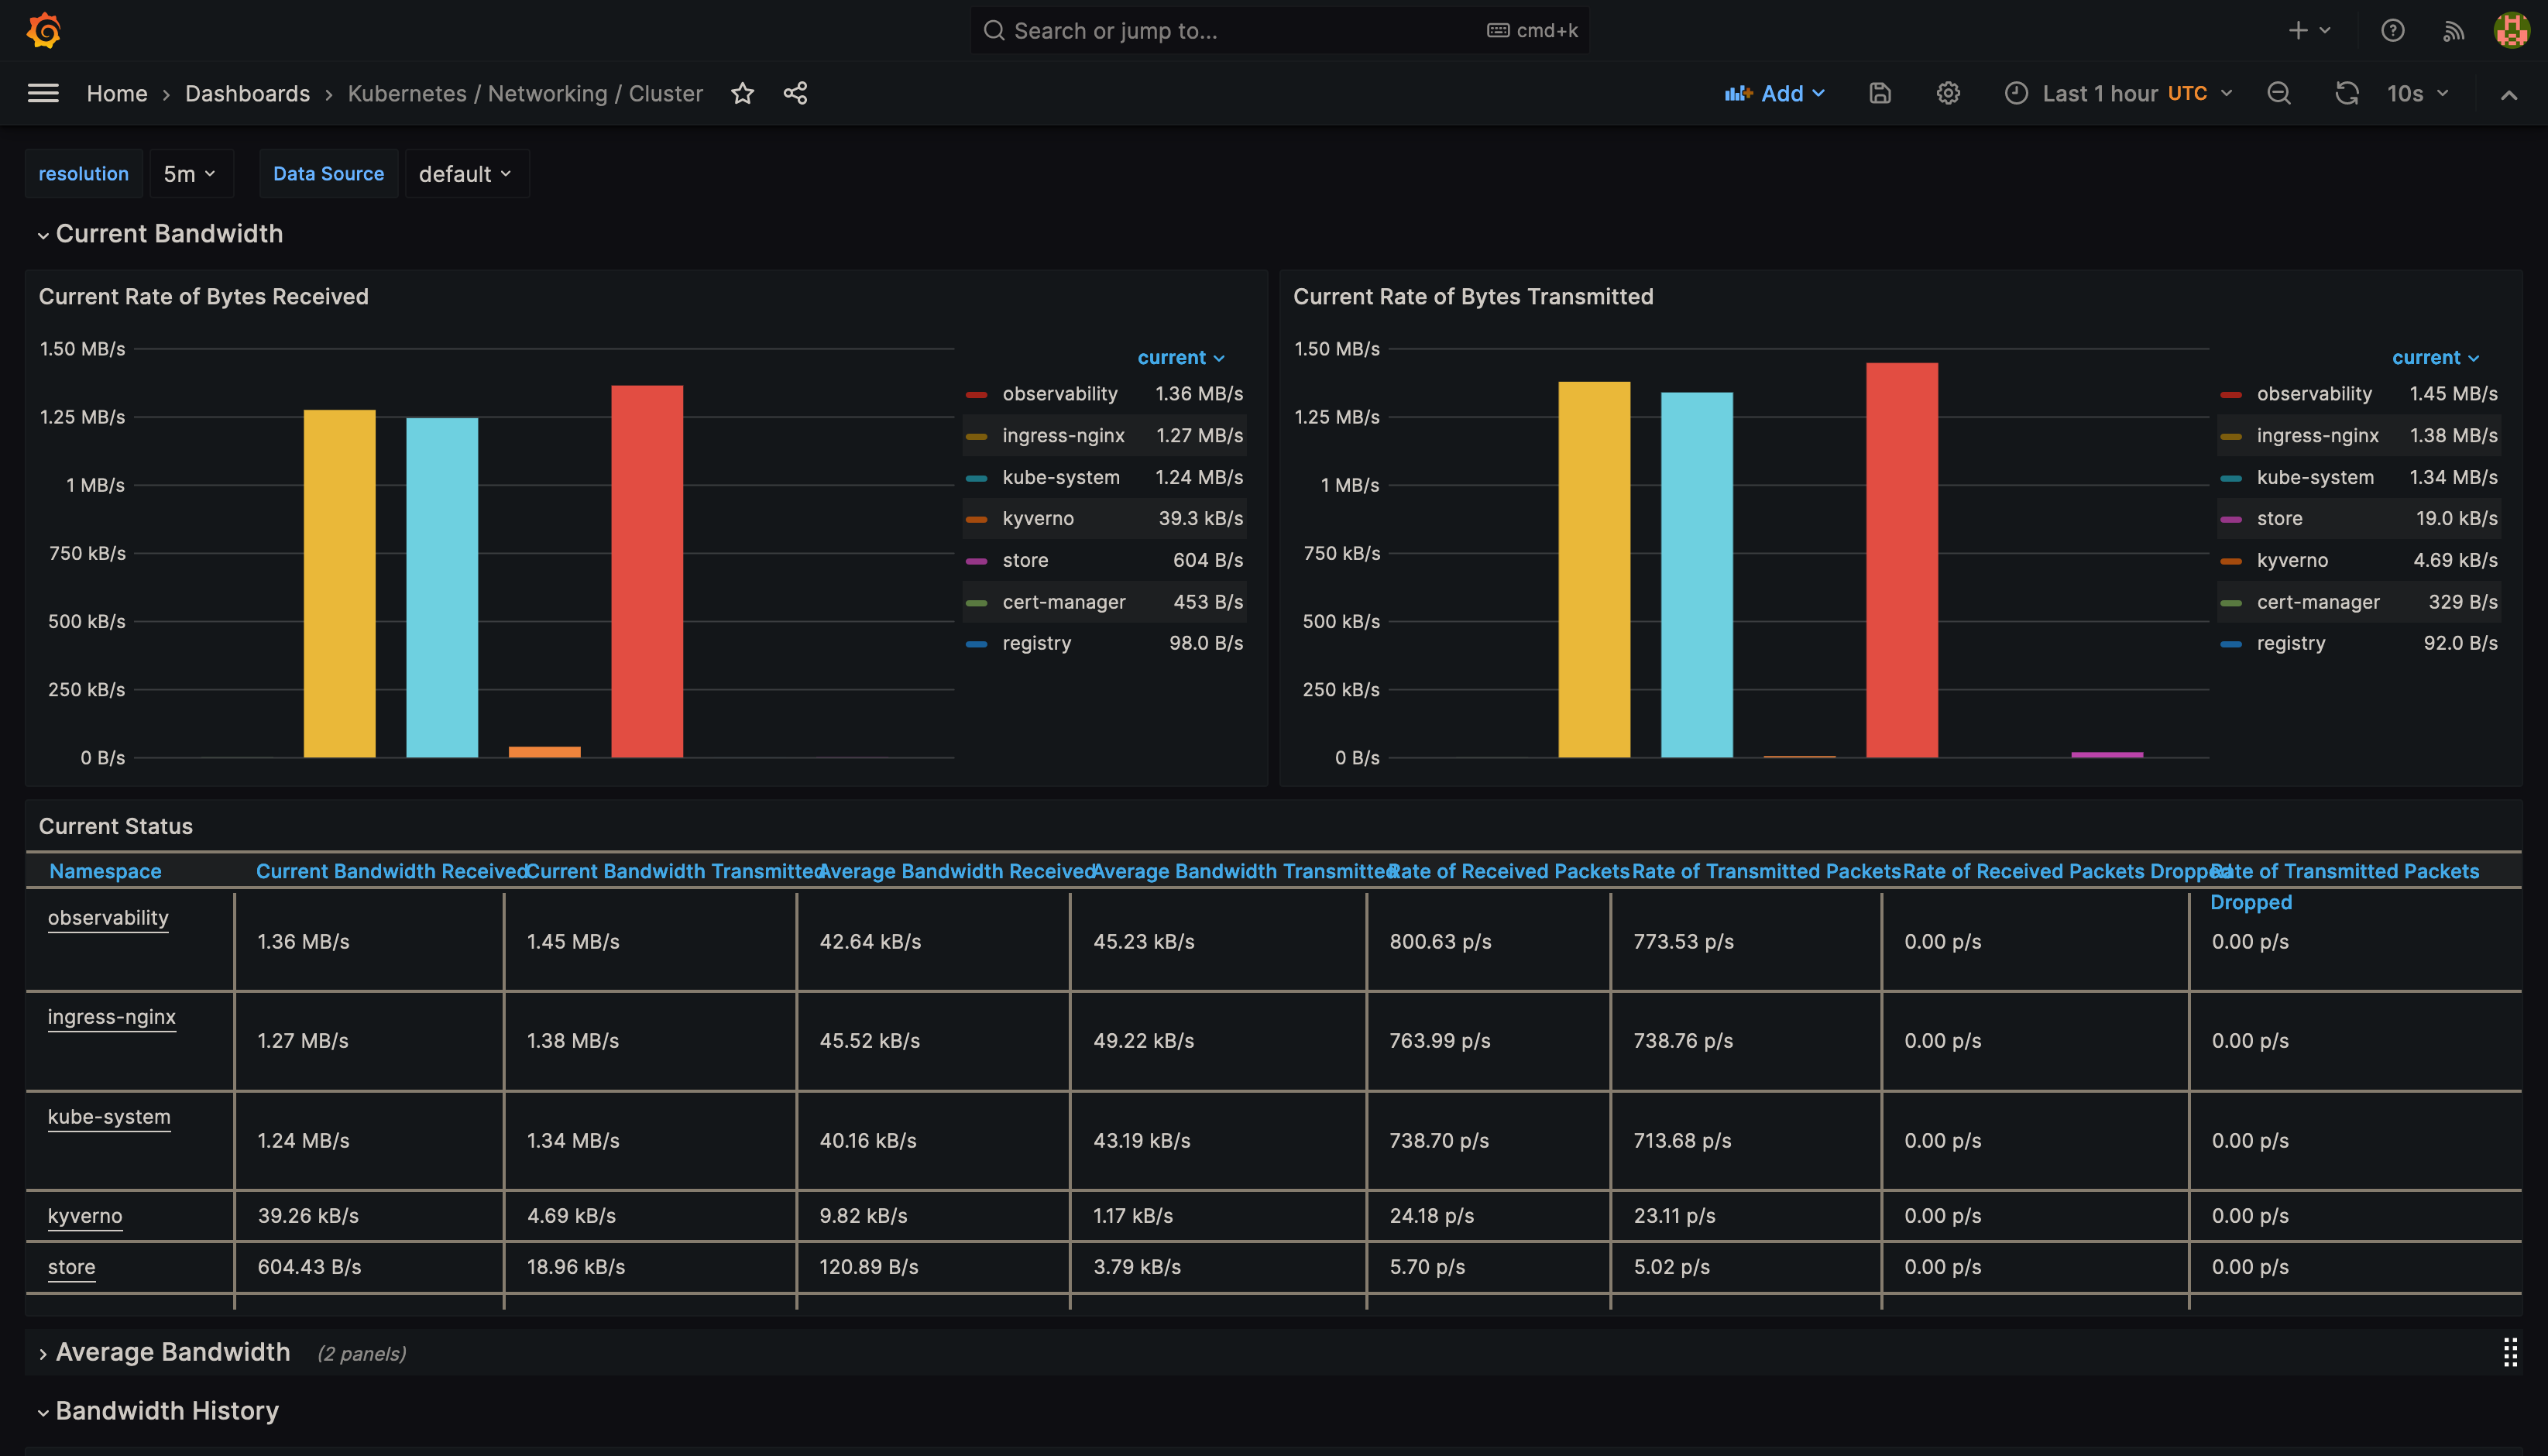
\includegraphics[width=\textwidth]{img/grafana-kubernetes-networking-cluster-dashboard}
%        \caption{Dashboard Kubernetes / Networking / Cluster}
%        \label{fig:grafana-kubernetes-networking-cluster-dashboard}
%    \end{figure}
%
%    \begin{figure}[H]
%        \centering
%        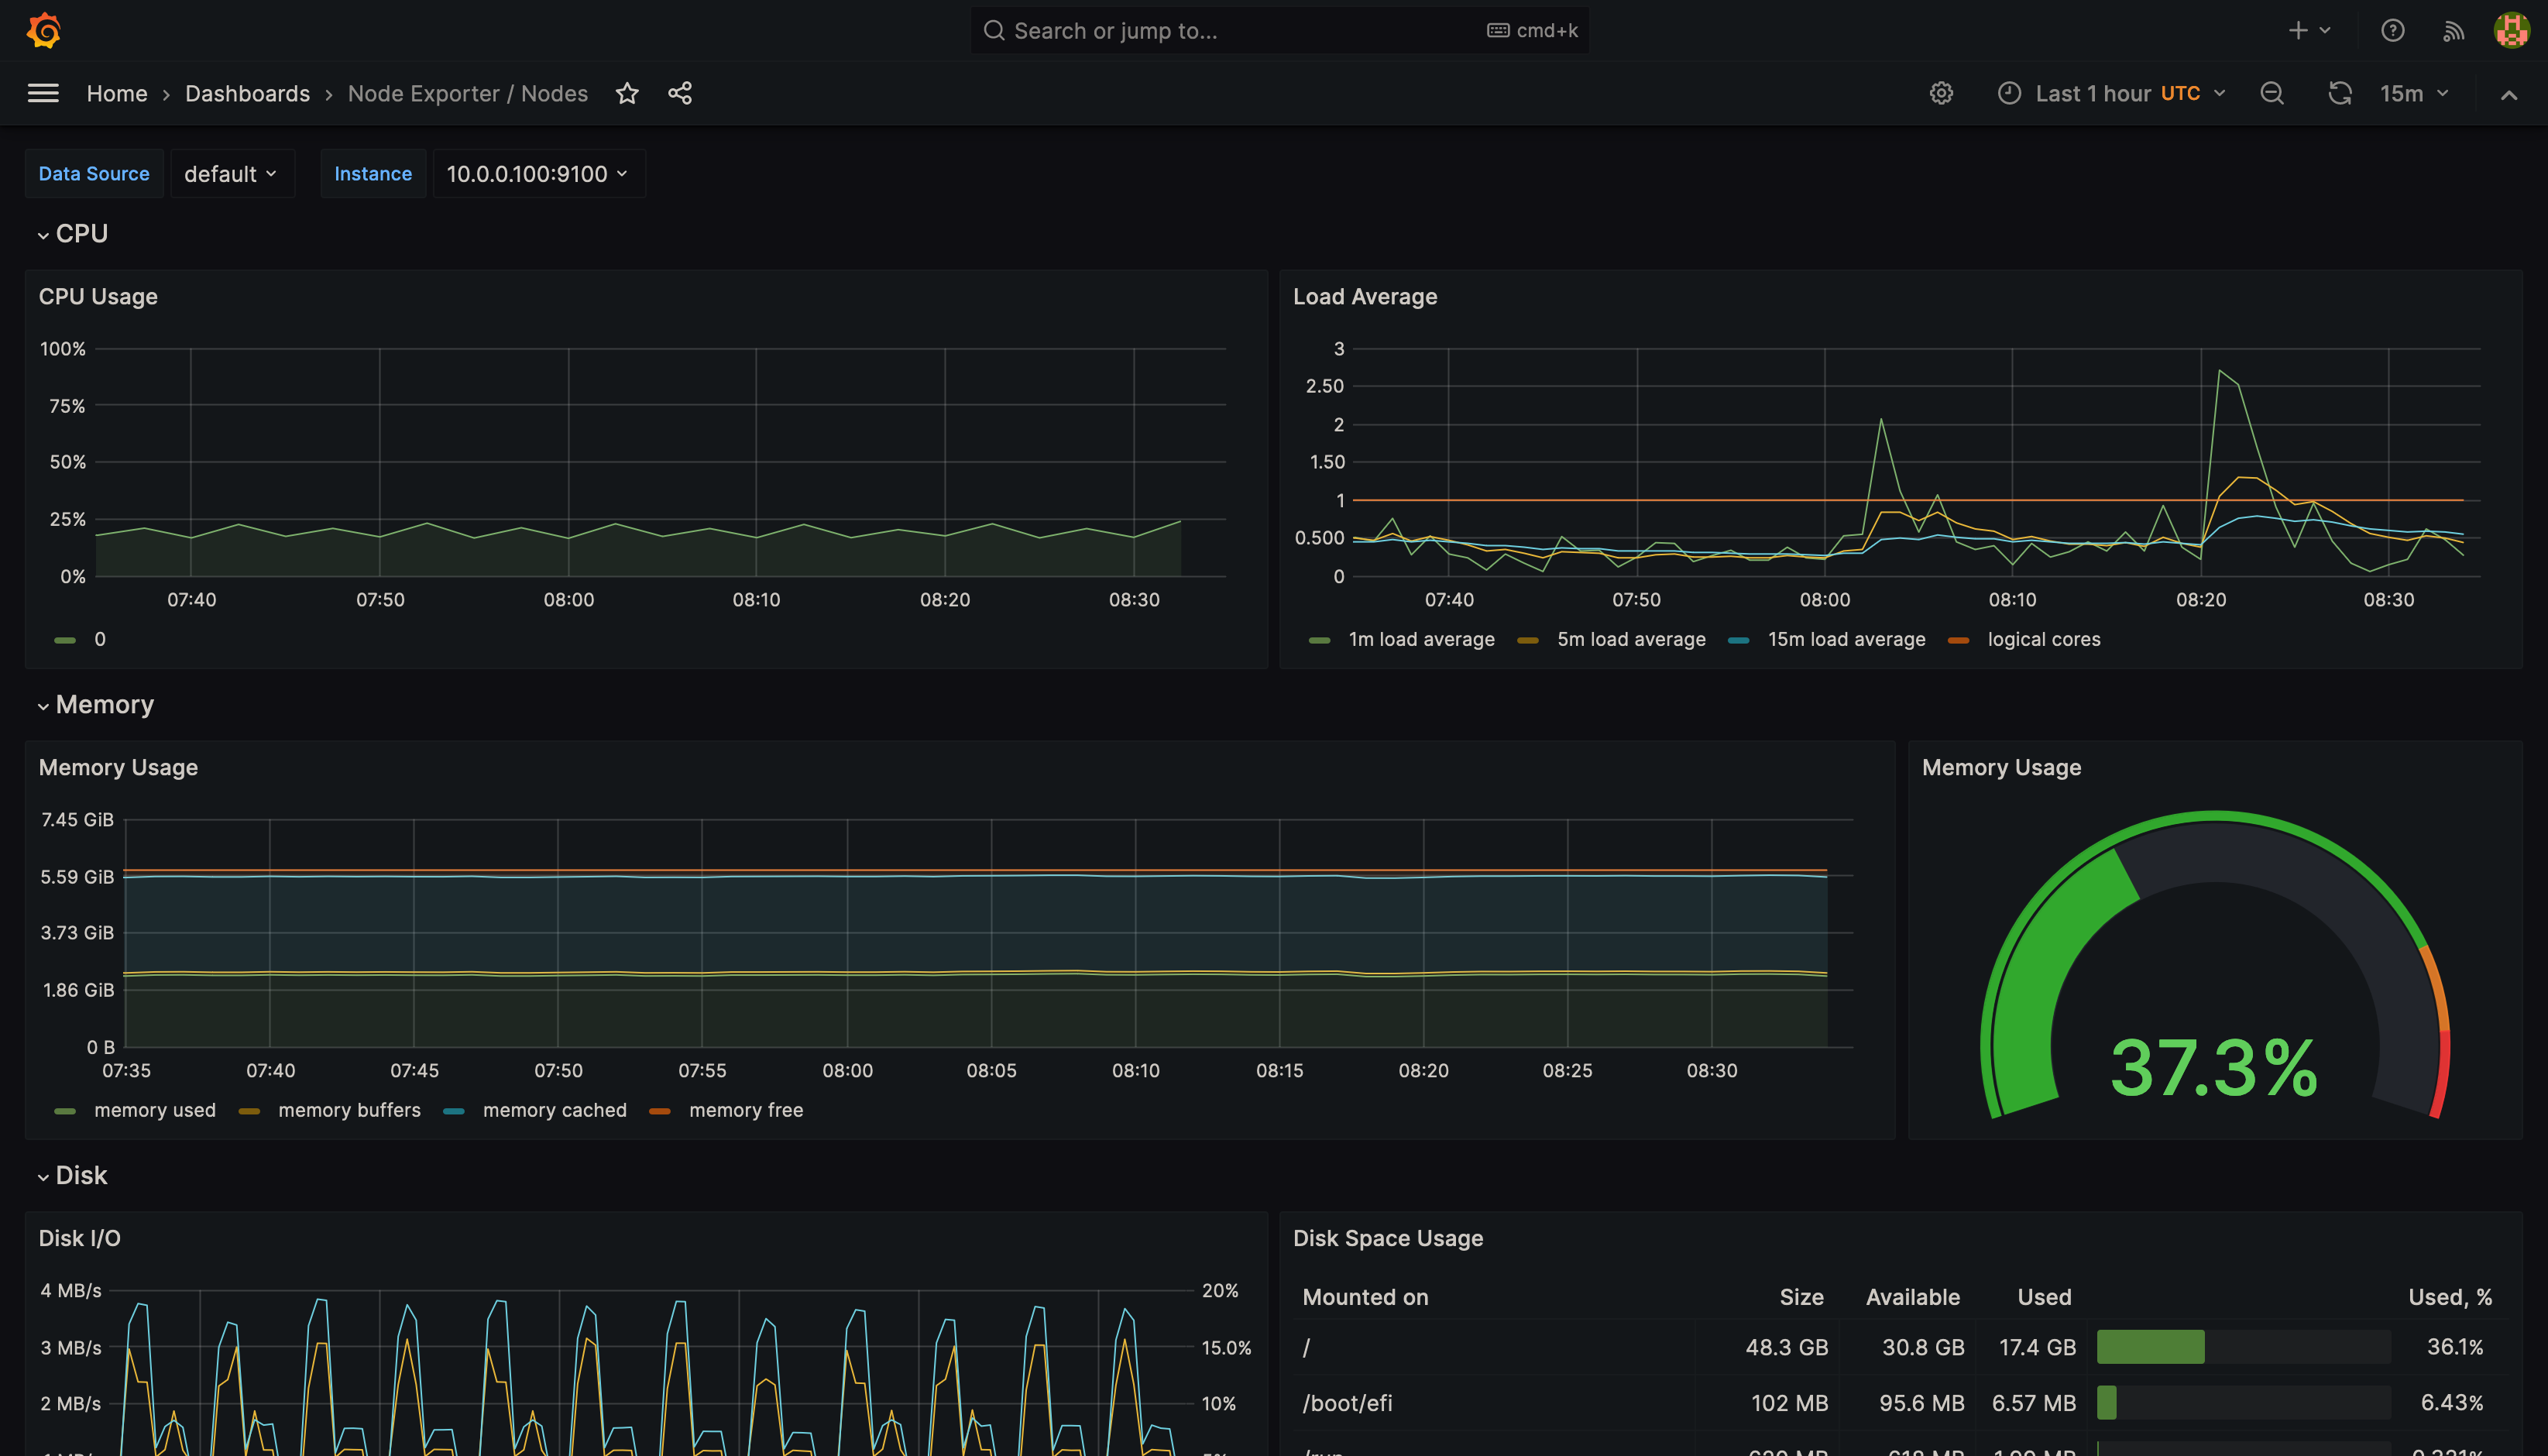
\includegraphics[width=\textwidth]{img/grafana-node-explorer-dashboard}
%        \caption{Dashboard Node Exporter / Nodes}
%        \label{fig:grafana-node-exlorer-dashboard}
%    \end{figure}
%\end{figure}

\subsection{Cert Manager}\label{subsec:cert-manager}

\todo{Cert Manager}

\begin{listing}[H]
    \begin{minted}{bash}
helm install cert-manager \
    --version v1.13.1 \
    --set installCRDs=true \
    --namespace cert-manager \
    --create-namespace \
    jetstack/cert-manager
    \end{minted}
    \caption{Polecenie instalujące pakiet jetstack/cert-manager}
    \label{lst:helm-install-cert-manager}
\end{listing}

\subsection{Docker Registry}\label{subsec:docker-registry}

\todo{Docker Registry}

\subsection{Store}\label{subsec:store}

\subsubsection{Przestrzeń nazw}

Przestrzenią nazw (ang. \emph{namespace}) nazywamy zbiór znaków (nazw) należących do jednego kontekstu.
Ich stosowanie umożliwia lepszą organizację i izolację zasobów, co przyczynia się do podniesienia bezpieczeństwa.
W środowisku Kubernetes przestrzenie nazw umożliwiają segmentację jednego klastra na mniejsze, logicznie wyizolowane jednostki.
Przestrzenie nazw mogą reprezentować środowiska różnych klientów (\emph{tenants}) lub środowiska na różnych poziomach (np. testowe i produkcyjne).

Opisywana platforma posiada przestrzeń nazw o nazwie \url{store}, która zawiera wszystkie elementy niezbędne do działania sklepu internetowego \url{store.tulski.com}.
Przestrzeń \url{store} została stworzona poprzez zaaplikowanie manifestu (zob. listing~\ref{lst:store-namespace}).

\begin{listing}[H]
    \inputminted[xleftmargin=20pt,linenos]{yaml}{code/store-namespace.yaml}
    \caption{Manifest tworzący przestrzeń nazw store}
    \label{lst:store-namespace}
\end{listing}

\subsubsection{Baza danych}\label{subsubsec:baza-danych}

Dane sklepu internetowego są fizycznie przechowywane na dyskach maszyn wirtualnych.
W CLI MicroK8s aktywowano dodatek Hostpath-Storage (zob. listing~\ref{lst:enable-hostpath-storage}), który udostępnia katalog hosta woluminom Kubernetes tj. PersistentVolumes.

\begin{listing}[H]
    \begin{minted}{bash}
microk8s enable hostpath-storage
    \end{minted}
    \caption{Polecenie aktywujące dodatek Hostpath-Storage}
    \label{lst:enable-hostpath-storage}
\end{listing}

\noindent Bazą danych jest PostgreSQL zainstalowany przy użyciu menadżera pakietów Helm (zob. rozdział~\ref{subsec:helm}).
Poleceniem \autoref{lst:helm-install-store-db} zainstalowano pakiet \url{bitnamicharts/postgresql} w przestrzeni \url{store}.

\begin{listing}[H]
    \begin{minted}{bash}
helm install store-db \
    --set auth.postgresPassword="<postgres-password>" \
    --set auth.username="store-db-admin" \
    --set auth.password="<password>" \
    --set auth.database="store" \
    --set metrics.enabled=true \
    --set metrics.serviceMonitor.enabled=true \
    --set metrics.serviceMonitor.namespace="observability" \
    --set metrics.serviceMonitor.labels.release="observability" \
    -n store \
    oci://registry-1.docker.io/bitnamicharts/postgresql
    \end{minted}
    \caption{Polecenie instalujące pakiet bitnamicharts/postgresql}
    \label{lst:helm-install-store-db}
\end{listing}

\subsubsection{Backend}

Backend, w rozumieniu architektury wielowarstwowej, pełni kluczowy element systemu informatycznego.
To warstwa stanowiąca zaplecze technologiczne, która w oparciu na zdefiniowanych regułach biznesowych, odpowiada za obsługę żądań klientów oraz przetwarza dane w sposób zapewniający ich spójność.

Serwer dostarczany przez projekt Medusa nie wymagał żadnych modyfikacji.
Jedynym wymogiem do jego uruchomienia było wybranie i dołączenie odpowiednich wtyczek (ang. \emph{plugins}) odpowiedzialnych za zarządzanie zamówieniami oraz obsługę płatności.
W tym celu zastosowano odpowiednio medusa-fulfillment-manual  i medusa-payment-manual (zob. \autoref{lst:medusa-config-fulfillment-payment}).
Obie te wtyczki można postrzegać jako atrapy (ang. \emph{mocks}), które umożliwiają funkcjonowanie serwera bez konieczności integracji z rzeczywistymi serwisami, takimi jak Stripe czy PayPal.

\begin{listing}[H]
    \begin{minted}[xleftmargin=20pt,linenos]{js}
const plugins = [
    `medusa-fulfillment-manual`,
    `medusa-payment-manual`,
    // ...
];
    \end{minted}
    \caption{Konfiguracja pluginów medusa-fulfillment-manual i medusa-payment-manual}
    \label{lst:medusa-config-fulfillment-payment}
\end{listing}

Aby backend mógł zostać uruchomiony w środowisku Kubernetes, koniecznie było jego skonteneryzowania.
Proces ten został zrealizowany przy użyciu narzędzia Docker (zob. podrozdział~\ref{subsec:docker}).
W tym celu stworzono plik Dockerfile (zob. listing~\ref{lst:code-dockerfile-backend}), który definiuje wszystkie kroki budowania obrazu kontenera.
Plik Dockerfile rozpoczyna się od określenia obrazu bazowego, czyli \url{node:18-alpine}.
Następnie, w kolejnych etapach \url{deps}, \url{builder} i \url{runner}, są kolejno instalowane zależności NPM, budowany jest kod aplikacji oraz przygotowywane jest środowisko uruchomieniowe serwera.

\begin{listing}[H]
    \inputminted[xleftmargin=20pt,linenos]{docker}{code/Dockerfile.backend}
    \caption{Plik Dockerfile.backend}
    \label{lst:code-dockerfile-backend}
\end{listing}

Backend został zainstalowany i skonfigurowany w środowisku Kubernetes.
Wszystkie komponenty i mechanizmy, które składają się na to wdrożenie, zostały przedstawione na rysunku~\ref{fig:kubernetes-backend}.
Wdrożenie odbywa się przez Deployment, co umożliwia automatyzację i skalowanie aplikacji.
Komunikacja z serwisem odbywa się poprzez NGINX Virtual Server, który szyfruje dane za pomocą certyfikatu TLS wygenerowanego przez Cert-Manager.
Backend korzysta z bazy danych PostgresSQL (zob. \autoref{subsubsec:baza-danych}).
Obserwowalność działania aplikacji zapewnia Prometheus Service Monitor.
Sekrety aplikacji są bezpiecznie zarządzane za pomocą mechanizmów Kubernetes Secrets.

\begin{figure}[H]
    \centering
    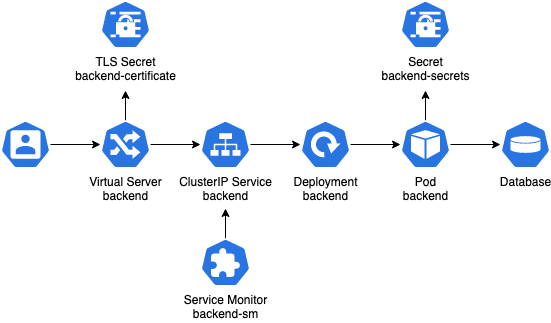
\includegraphics[width=\textwidth]{img/kubernetes-backend}
    \caption{Backend w środowisku Kubernetes}
    \label{fig:kubernetes-backend}
\end{figure}

\subsubsection{Panel administratora}

Panel administratora to kolejny element rozbudowanego ekosystemu Medusa, który jest dostarczany w formie wtyczki (ang. \emph{plugin}).
Panel stanowi graficzny interfejs dla Admin REST API. Jego zastosowanie umożliwia łatwe zarządzanie produktami, zamówieniami oraz ustawieniami sklepu.

Wtyczka panelu administratora, skonfigurowana w plikach serwera backend (zob. listing~\ref{lst:medusajs-admin-plugin}), może być uruchomiona równolegle z backendem, lub jako niezależny serwer.
Zdecydowano się na drugą opcję, ponieważ pozwala ona na niezależne skalowanie obu aplikacji.

\begin{listing}[H]
        \begin{minted}[xleftmargin=20pt,linenos]{js}
const plugins = [
    {
        resolve: "@medusajs/admin",
        options: { /* ... */ },
    },
    // ...
];
        \end{minted}
    \caption{Dołączenie wtyczki @medusajs/admin}
    \label{lst:medusajs-admin-plugin}
\end{listing}

Panel administratora jest budowany do postaci statycznych plików HTML, CSS i JavaScript, które następnie są hostowane przez serwer NGINX (zob. listing~\ref{lst:medusajs-admin-dockerfile}).

\begin{listing}[H]
    \inputminted[xleftmargin=20pt,linenos]{docker}{code/Dockerfile.admin}
    \caption{Plik Dockerfile panelu administratora}
    \label{lst:medusajs-admin-dockerfile}
\end{listing}

Panel administratora w środowisku Kubernetes funkcjonuje jako osobna jednostka wdrożeniowa, niezależna od backendu.
Wykorzystuje NGINX Virtual Server z szyfrowaniem TLS. Certyfikat jest generowany przez Cert-Manager.
Architektura obejmuje service oraz deployment z jednym podem, co przedstawiano na rysunku~\ref{fig:kubernetes-admin}.

\begin{figure}[H]
    \centering
    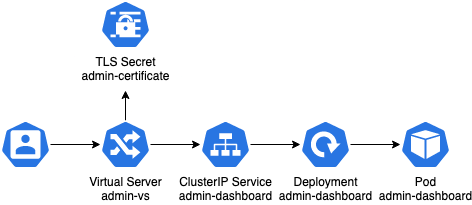
\includegraphics[width=0.9\textwidth]{img/kubernetes-admin-panel}
    \caption{Panel administratora w środowisku Kubernetes}
    \label{fig:kubernetes-admin}
\end{figure}

\subsubsection{Witryna internetowa}

Witryna internetowa, będąca warstwą prezentacyjną systemu, odgrywa kluczową rolę w interakcji z klientem końcowym.
Główny zadaniem tej witryny jest prezentacja oferowanych produktów oraz umożliwienie użytkownikom przeprowadzenia procesu zakupowego.
Projekt Medusa dostarcza szablon witryny sklepu internetowego w formie osobnego projektu o nazwie Storefront.
Storefront, jako graficzny interfejs dla Store REST API, stanowi integralną część reszty systemu Medusa.

Witryna internetowa, analogicznie do części serwerowej oraz panelu administratora, została zintegrowana w strukturze całej platformy poprzez proces skonteneryzowania i wdrożenia w środowisku Kubernetes (zob. rysunek~\ref{fig:kubernetes-storefront}).

\begin{figure}[H]
    \centering
    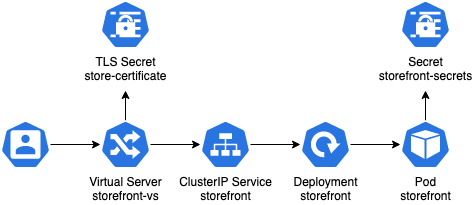
\includegraphics[width=\textwidth]{img/kubernetes-storefront}
    \caption{Witryna internetowa w środowisku Kubernetes}
    \label{fig:kubernetes-storefront}
\end{figure}

Rysunek~\ref{fig:storefront-homepage} przedstawia stronę domową sklepu, akcentując powód jego powstania, czyli niniejszą pracę dyplomową.
Natomiast rysunek~\ref{fig:storefront-products} ilustruje stronę z produktami, ukazując sposób prezentacji asortymentu.
Obie strony razem podkreślają znaczenie estetyki i funkcjonalności w interfejsie użytkownika sklepu internetowego.

\begin{figure}[p]
    \begin{figure}[H]
        \centering
        \fbox{\includegraphics[width=\textwidth]{img/storefront-homepage}}
        \caption{Strona domowa sklepu internetowego}
        \label{fig:storefront-homepage}
    \end{figure}

    \begin{figure}[H]
        \centering
        \fbox{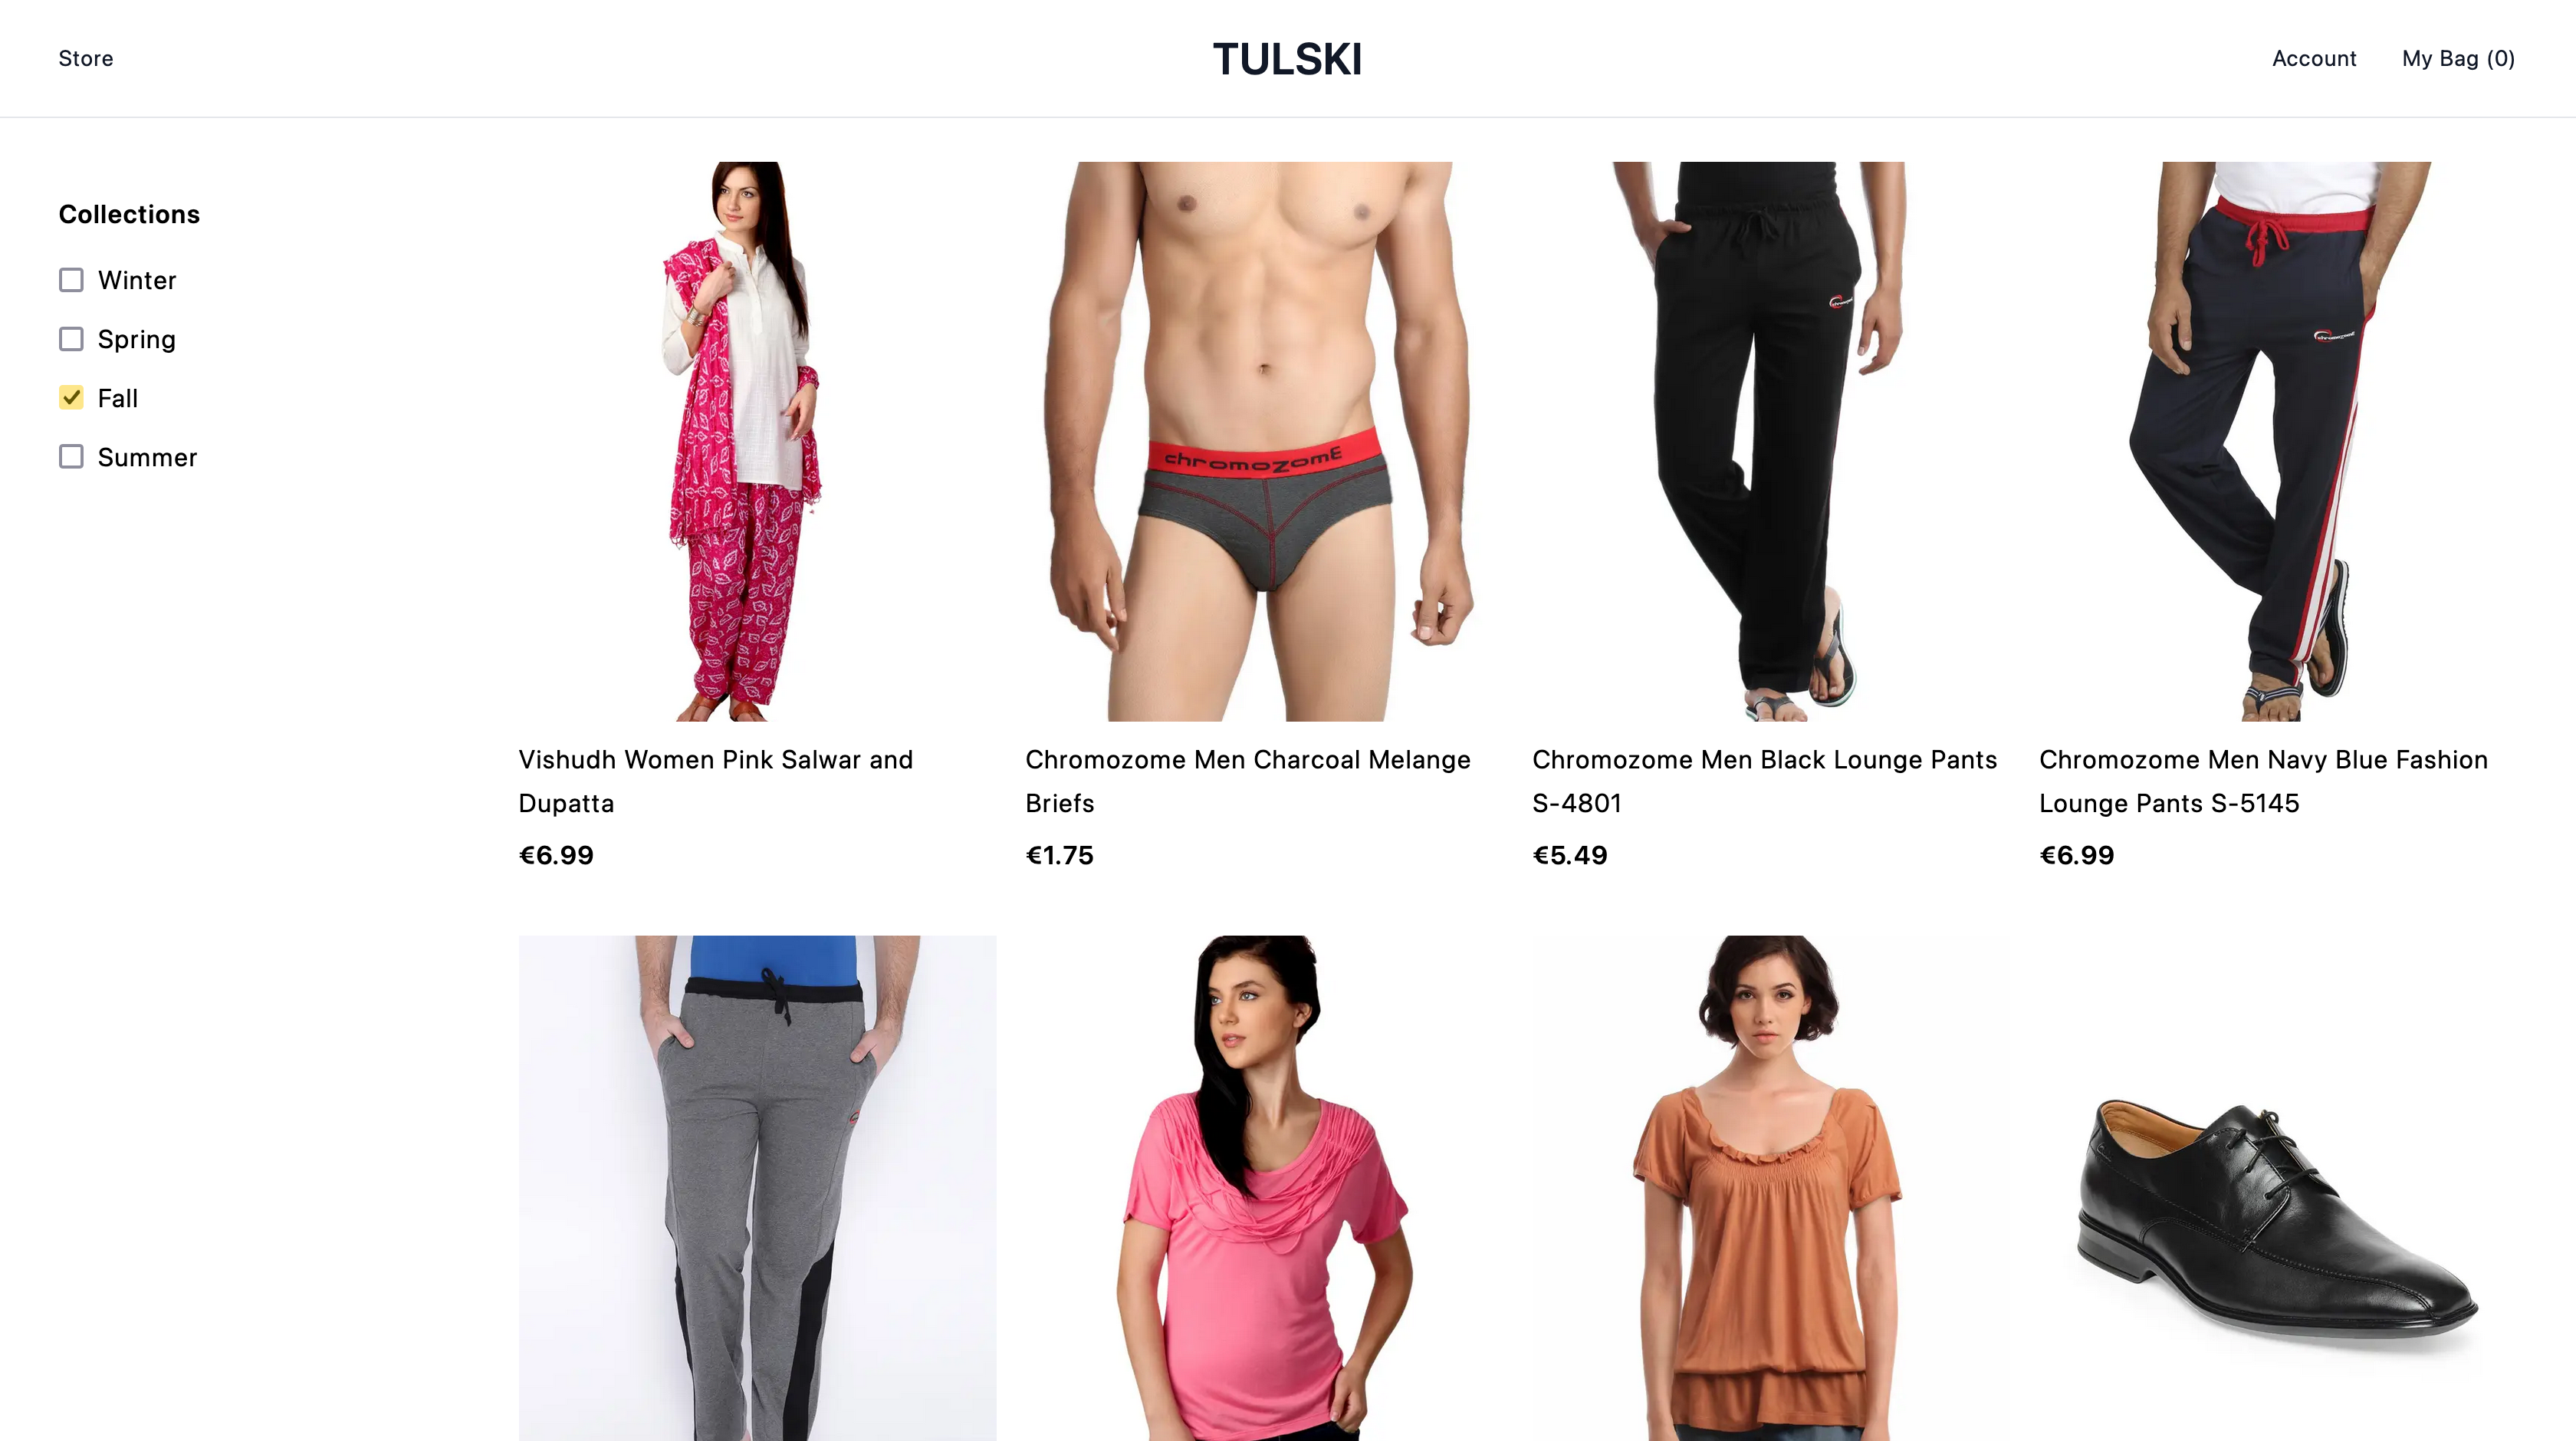
\includegraphics[width=\textwidth]{img/storefront-products}}
        \caption{Strona z produktami sklepu internetowego}
        \label{fig:storefront-products}
    \end{figure}
\end{figure}

\subsubsection{Populacja danych}

\todo{Populacja danych}